\documentclass[10pt,openany]{article}
\usepackage{ctex} 
\usepackage{geometry,graphicx,xcolor,color}
\geometry{
	a4paper,
	top=25.4mm, bottom=25.4mm,
	left=20mm, right=20mm,
	headheight=2.17cm,
	headsep=4mm,
	footskip=12mm
}
\usepackage{pifont}
\usepackage[all,pdf]{xy}
\usepackage{amssymb,amsmath,mathrsfs}             
\usepackage{mathpazo}
\usepackage[nofontspec]{newpxtext}
\usepackage{array}
\usepackage{amsmath}
\usepackage{amssymb}
\usepackage{enumerate}
\usepackage{amsthm}
\usepackage{bm}
\usepackage{mathtools}
\usepackage{mathrsfs}
\usepackage{tcolorbox}
\usepackage{indentfirst}
\usepackage{setspace}
\usepackage{subfigure} 
\usepackage{tkz-fct}
\usetikzlibrary{calc,intersections,through,backgrounds,3d}
\usepackage{tkz-euclide}
\usepackage{pgfplots}
\usepackage{booktabs}
\usepackage{float}
\usepackage[graphicx]{realboxes}
\usepackage{fancyhdr}

\definecolor{winered}{rgb}{0.5,0,0}
\definecolor{structurecolor}{RGB}{122,122,142}
\definecolor{main}{HTML}{3D445F}
\definecolor{second}{HTML}{627581}
\definecolor{third}{HTML}{9D8798}


\usepackage{hyperref}
\hypersetup{colorlinks = true, linktoc=all, linkcolor=black, urlcolor=winered}


\usepackage{amsthm}
% 设定颜色(假设你在别处定义了 \color{main} 等)
\usepackage{xcolor}

% 定义定理风格
\usepackage{amsthm}
\newtheoremstyle{defstyle}
{0.3cm}{0.3cm}{\fangsong}{-1cm}{\bfseries\color{main}}{}{0.5em}
{\indent 【\thmname{#1} \thmnumber{#2}】\ifthenelse{\equal{#3}{}}{}{~\thmnote{(#3)}}}

\newtheoremstyle{thmstyle}
{0.3cm}{0.3cm}{\kaishu}{-1cm}{\bfseries\color{second}}{}{0.5em}
{\indent 【\thmname{#1} \thmnumber{#2}】\ifthenelse{\equal{#3}{}}{}{~\thmnote{(#3)}}}

\newtheoremstyle{prostyle}
{0.3cm}{0.3cm}{\kaishu}{-1cm}{\bfseries\color{third}}{}{0.5em}
{\indent 【\thmname{#1} \thmnumber{#2}】\ifthenelse{\equal{#3}{}}{}{~\thmnote{(#3)}}}

\theoremstyle{thmstyle} %theorem style
\newtheorem{theorem}{定理}[subsection]
\theoremstyle{defstyle} % definition style
\newtheorem{definition}[theorem]{定义}
\newtheorem{lemma}[theorem]{引理}
\newtheorem{corollary}[theorem]{推论}
\theoremstyle{prostyle} % proposition style
\newtheorem{proposition}[theorem]{命题}
\newtheorem{example}[theorem]{例}
\newtheorem{remark}[theorem]{注}

\renewenvironment{proof}[1][证明]{\par\underline{\textbf{#1.}} \;\fangsong}{\qed\par}
\newenvironment{solution}{\par\underline{\textbf{解.}} \;\fangsong}{\qed\par}
\newcommand{\intro}[1]{\rightline{\parbox[t]{5cm}{\footnotesize \fangsong\quad\quad #1 }}}


\usepackage{titlesec, titletoc}
\linespread{1.2} 				
\usepackage{fancyhdr}
\fancyhf{}
\renewcommand{\headrule}{\color{structurecolor}\hrule width\textwidth}
\pagestyle{fancy}
\renewcommand{\headrulewidth}{1pt}
\fancypagestyle{plain}{\renewcommand{\headrulewidth}{0pt}\fancyhf{}\renewcommand{\headrule}{}}

\fancyhead[c]{\color{structurecolor}\kaishu\rightmark}
\fancyfoot[c]{\color{structurecolor}\small\thepage}


\titleformat{\section}[frame]{\normalfont\color{structurecolor}}{\footnotesize \enspace \large \textcolor{structurecolor}{\S \,\thesection}\enspace}{6pt}{\Large\filcenter \bf \kaishu }


\titleformat{\subsection}[hang]{\bfseries}{\large\bfseries\color{structurecolor}\thesubsection\enspace}{1pt}{\color{structurecolor}\large\bfseries\filright}

\titleformat{\subsubsection}[hang]{\bfseries}{\large\bfseries\color{structurecolor}\thesubsubsection\enspace}{1pt}{\color{structurecolor}\large\bfseries\filright}

\usepackage{titling}
\renewcommand*{\maketitle}{
	\begin{titlepage}
		\newgeometry{margin = 0in}
		\parindent=0pt
		\includegraphics[width=\linewidth]{cover.png}
		\vfill
		\begin{center}
			\parbox{0.618\textwidth}{
				\hfill {\bfseries \Huge \thetitle} \\[0.6pt]  
				\rule{0.618\textwidth}{4pt} \\ 
			}
		\end{center}
		\vfill
		\begin{center}
			\parbox{0.618\textwidth}{
				\hfill\Large
				\kaishu 
				\begin{tabular}{r|}
					\textbf{2025 Summer} \\
					作者:\theauthor \\ 
					时间:\thedate \\
				\end{tabular}
			}
		\end{center}
		\vfill
		\begin{center}
			\parbox[t]{0.7\textwidth}{\centering \kaishu}
		\end{center}
		\vfill
	\end{titlepage}
	\restoregeometry
	\thispagestyle{empty}
}

\newcommand{\oneb}{\underline{\hspace{1em}}\hspace{0.001em}}
\newcommand{\twob}{\oneb\oneb}
\newcommand{\fourb}{\twob\twob}
\newcommand{\tenb}{\twob\twob\twob\twob\twob}
\newcommand{\tideparallel}{%  
	\mathrel{%  
		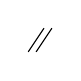
\begin{tikzpicture}[scale=0.2, baseline={([yshift=-0.5ex]current bounding box.center)}]  
			\draw[thin] (0,0) -- (1,1.5);  
			\draw[thin] (0.5,0) -- (1.5,1.5);  
		\end{tikzpicture}%  
	}%  
}  
\newcommand{\fourch}[4]
{\\[3pt]
	\begin{tabular}
		{*{4}{@{}p{4cm}}}
		A.~#1 & B.~#2 & C.~#3 & D.~#4
	\end{tabular}	
}
\newcommand{\fourchh}[4]
{\\[5pt]
	\begin{tabular}
		{*{4}{@{}p{20cm}}}
		A.~#1 \\[5pt] B.~#2 \\[5pt] C.~#3 \\[5pt] D.~#4
	\end{tabular}	
}
\newcommand{\fourchhh}[4]
{\\[3pt]
	\begin{tabular}
		{*{4}{@{}p{7.5cm}}}
		A.~#1 & B.~#2 \\[2pt] C.~#3 & D.~#4
	\end{tabular}	
}
\newcommand{\independent}{\perp\!\!\!\perp}
\everymath{\displaystyle}
\allowdisplaybreaks




\begin{document}

\pagestyle{fancy}
\lhead{Lecture 1}
\chead{illusion \& FzRainD}
\rhead{\today}

\section{Guass-Jordan 消元法和矩阵运算}
\subsection{初等变换和 Guass-Jordan 消元法}
\label{1.1}
代数学起源于数系的扩充,方程的求解. 而在今天,代数学的主要研究对象集中在代数系统及其之间的态射上,在高等代数 I 的后半部分,我们将集中研究一类最简单的代数系统及其态射,线性空间和线性映射,更确切地说,我们大多时候只关注有限维线性空间. 无限维线性空间理论会在泛函分析课程进一步讨论.

对方程而言,我们不仅希望找到是否有解的判定准则,更希望能找到一套普适的算法在方程有解时计算出所有解. 高等代数的一个重要组成部分是线性代数. 所谓"线性",指的是加法和数乘两个运算. 往一般了说,加法指的是一个集合关于该运算构成 Abel 群,而数乘,则可以看成是某个交换环在这个 Abel 群上的作用,并且需要满足运算间的若干协调性. 不过,我们现在不关心这些. 我们的起点不过就是高中所学的平面 \( \mathbb{R}^2:=\{(a,b) \mid a,b \in \mathbb{R} \} \),以及空间 \( \mathbb{R}^3:=\{ (a,b,c) \mid a,b,c \in \mathbb{R} \} \),乃至这一概念的自然推广: \( n \) 维向量空间
\[ \mathbb{R}^n:=\{ (x_1,x_2,\cdots,x_n) \mid x_1,\cdots,x_n \in \mathbb{R} \}. \]

这里的线性运算指的是
\begin{enumerate}[(1)]
	\item 向量的加法: \( (x_1,\cdots,x_n)+(y_1,\cdots,y_n)=(x_1+y_1,\cdots,x_n+y_n) \);
	\item \( \mathbb{R} \) 中的数与向量的数乘: \( k(x_1,\cdots,x_n)=(kx_1,\cdots,kx_n), \; k \in \mathbb{R} \).
\end{enumerate} 

在线性运算下,线性方程组为我们重要的一个研究对象. 设 \( x_1,\cdots,x_n \) 为 \( n \) 个未定元,给出 \( m \) 个关于 \( x_1,\cdots,x_n \) 的线性方程,并联立,即
\begin{equation}
	\left\{\begin{array}{l}
		a_{11}x_1+a_{12}x_2+\cdots+a_{1n}x_n=b_1, \\
		a_{21}x_1+a_{22}x_2+\cdots+a_{2n}x_n=b_1, \\
		\qquad \vdots \\
		a_{m1}x_1+a_{m2}x_2+\cdots+a_{mn}x_n=b_m.
	\end{array}\right.
	\label{linequ.}
\end{equation}


其中 \( a_{ij}, b_i \in \mathbb{R} \ (1 \leq i \leq m,\; 1 \leq j \leq n) \). 对 \( m,n \) 的大小关系,我们并不关心,只要求它们均有限即可. 我们在中学阶段已经学习过 \( n=m=2 \) 以及 \( n=m=3 \) 这两种特殊情形的线性方程组. 所用的方法无非是代入法和加减消元法. 但这两种方法对 \( n \) 个变量的情形就有些困难了,因为很多时候,加减无法实现消元的效果; 而代入法对求解的难度也几乎于事无补. 为了更自然的引出下面有关求解线性方程组的 Guass-Jordan 消元法,我们从几个例子开始.

\begin{example}
	求解线性方程组
	\[
	(I) \left\{
	\begin{array}{l}
		x_1 + 3x_2 + x_3 = 2, \\
		3x_1 + 4x_2 + 2x_3 = 9, \\
		-x_1 - 5x_2 + 4x_3 = 10, \\
		2x_1 + 7x_2 + x_3 = 1.
	\end{array}
	\right.
	\]
	\label{1.1.1}
\end{example}

\begin{solution}
	这是一个 \( m=4, \; n=3 \) 的方程组. 为了求出未知数的值,我们发现如果能设法消去 \( x_1,x_2 \),那么最后只剩下 \( x_3=? \) 的形式,再回代方程,得到关于 \( x_1,x_2 \) 的方程组,相同的方法可以依次解出 \( x_2,x_1 \). 我们用 \( (i) \) 表示这个方程的第 \( i \) 行. 现在我们希望用 \( (1) \) 消去 \( (2),(3),(4) \) 中所有的 \( x_1 \) 项. 你可能会疑惑,为什么要用 \( (1) \),而不是 \( (2) \) 或者其他行. 观察到此时 \( (1) \) 中 \( x_1 \) 的系数为 \( 1 \),如果我们将 \( (1) \times (-a_{i1}) \) 加到第 \( i \) 行上,那就可以把第 \( i \) 行中的 \( x_1 \) 消去了. 如果使用 \( (2) \) 完成这个步骤,那就会涉及除法,增加我们的计算量,可行但没有用 \( (1) \) 来的方便. 
	
	今后我们用 \( (j)+(i) \times k \) 表示用第 \( i \) 个方程的 \( k \) 倍加到第 \( j \) 行上. 那么我们得到
	\[ (\text{I}) \left\{
	\begin{array}{l}
		x_1 + 3x_2 + x_3 = 2, \\
		3x_1 + 4x_2 + 2x_3 = 9, \\
		-x_1 - 5x_2 + 4x_3 = 10, \\
		2x_1 + 7x_2 + x_3 = 1.
	\end{array}
	\right. \leadsto (\text{II}) \left\{
	\begin{array}{l}
		x_1 + 3x_2 + x_3 = 2, \\
		-5x_2 - x_3 = 3, \qquad (2)+(1) \times (-3) \\
		-2x_2 + 5x_3 = 12, \qquad (3)+(1) \times 1 \\
		x_2 - x_3 = -3.\qquad (4)+(1) \times (-2)
	\end{array}
	\right.\]
	
	这完美实现了第一步消元,但是有一个问题. 方程 (II) 的解是方程 (I) 的解吗? 我们知道如果 \( (x_1,x_2,x_3) \) 适合方程 (I),那么其必定适合方程 (II). 反之,成立吗? 实行操作 \( (2)-(1) \times (-3), \; (3)-(1) \times 1, \; (4)-(1) \times (-2) \),我们就能将方程 (II) 转化为方程 (I). 这事实上回答了我们的问题,因为这说明如果 \( (x_1,x_2,x_3) \) 适合方程 (II),那么其必定适合方程 (I). 也即
	
	\begin{center}
		\fbox{方程 (I) 和方程 (II) 是同解的方程组!}
	\end{center}
	
	下面我们就可以放心地求解方程 (II). 这时,如果还希望进行我们刚才类似的消元操作,那么方程 (II) 的 \( (2) \) 这个方程不太好,\( x_2 \) 的系数为 \( -5 \). 但是我们发现 \( (4) \) 中  \( x_2 \) 前面的系数为 \( 1 \). 于是打算将第 2 行与第 4 行互换,这个操作简单记作 \( [(2),(4)] \).
	
	\[ (\text{II}) \left\{
	\begin{array}{l}
		x_1 + 3x_2 + x_3 = 2, \\
		-5x_2 - x_3 = 3, \\
		-2x_2 + 5x_3 = 12, \\
		x_2 - x_3 = -3.
	\end{array}
	\right. \overset{[(2),(4)]}{\leadsto} (\text{III}) \left\{
	\begin{array}{l}
		x_1 + 3x_2 + x_3 = 2, \\
		x_2 - x_3 = -3, \\
		-2x_2 + 5x_3 = 12, \\
		-5x_2 - x_3 = 3.
	\end{array}
	\right. \]
	
	这时候方程 (II) 与方程 (III) 同解就是显然的了. 接下来,类似刚才的操作有
	
	 \begin{align*}
		(\text{III}) \left\{
		\begin{array}{l}
			x_1 + 3x_2 + x_3 = 2, \\
			x_2 - x_3 = -3, \\
			-2x_2 + 5x_3 = 12, \\
			-5x_2 - x_3 = 3.
		\end{array}
		\right. &\leadsto (\text{IV}) \left\{
		\begin{array}{l}
			x_1 + 3x_2 + x_3 = 2, \\
			x_2 - x_3 = -3\\
			3x_3 = 6 , \qquad (3)+(2) \times 2 \\
			-6x_3 = -12. \qquad (4)+(2) \times 5
		\end{array}
		\right. \\
		&\leadsto (\text{V}) \left\{
		\begin{array}{l}
			x_1 + 3x_2 + x_3 = 2, \\
			x_2 - x_3 = -3, \\
			3x_3 = 6, \\
			0 = 0. \qquad (4)+(3) \times 2
		\end{array}
		\right.
	\end{align*}  
	
	
	为了得到 \( x_3 \) 的具体数值,将方程 (V) 中的 \( (3) \) 变为原来的 \( 1/3 \) 倍,记作 \( (3) \times (1/3) \). 那么
	
	 \begin{align*}
		 (\text{V}) \left\{
		\begin{array}{l}
			x_1 + 3x_2 + x_3 = 2, \\
			x_2 - x_3 = -3, \\
			3x_3 = 6, \\
			0 = 0. 
		\end{array}
		\right. &\leadsto (\text{VI}) \left\{
		\begin{array}{l}
			x_1 + 3x_2 + x_3 = 2, \\
			x_2 - x_3 = -3, \\
			x_3 = 2, \qquad (3) \times (1/3) \\
			0 = 0.
		\end{array}
		\right.\\
		&\leadsto (\text{VII}) \left\{
		\begin{array}{l}
			x_1 + 3x_2 = 0, \qquad (1)+(3) \times (-1) \\
			x_2 = -1, \qquad (2)+(3) \times 1\\
			x_3 = 2, \\
			0 = 0.
		\end{array}
		\right.\\
		&\leadsto (\text{VIII}) \left\{
		\begin{array}{l}
			x_1 = 3, \qquad (1)+(2) \times (-3) \\
			x_2 = -1, \\
			x_3 = 2, \\
			0 = 0.
		\end{array}
		\right.
	\end{align*}  
	
	其中方程 (V) 和方程 (VI) 是同解方程,这一点是不言自明的. 于是我们得到原方程有唯一解 \( (x_1,x_2,x_3)=(3,-1,2) \).
	
	(\textbf{另一种操作}) 在上面的计算中,我们先从上到下处理方程,使得最后一个方程只剩下 \( x_3 \) 一个变量,然后再回代到前面的方程中. 我们也可以在消去 \( x_2 \) 和 \( x_3 \) 这两个变量的过程中,兼顾前面的方程,一步到位. 回到方程 (III),
	
	\begin{align*}
		(\text{III}) \left\{
		\begin{array}{l}
			x_1 + 3x_2 + x_3 = 2, \\
			x_2 - x_3 = -3, \\
			-2x_2 + 5x_3 = 12, \\
			-5x_2 - x_3 = 3.
		\end{array}
		\right. &\leadsto  \left\{
		\begin{array}{l}
			x_1 + 4x_3 = 11, \qquad (1)+(2) \times (-3)\\
			x_2 - x_3 = -3, \\
			3x_3 = 6, \qquad (3)+(2) \times 2 \\
			-6x_3 = -12. \qquad (4)+(2) \times 5 
		\end{array}
		\right. \\
		&\leadsto  \left\{
		\begin{array}{l}
			x_1 + 4x_3 = 11, \\
			x_2 - x_3 = -3, \\
			x_3 = 2, \qquad (3) \times (1/3) \\
			-6x_3 = -12. 
		\end{array}
		\right. \\
		&\leadsto  \left\{
		\begin{array}{l}
			x_1  = 3, \qquad (1)+(3) \times (-4)\\
			x_2  = -1, \qquad (2)+(3) \times 1 \\
			x_3 = 2,  \\
			0=0. \qquad (4)+(3) \times 2 
		\end{array}
		\right. \\
	\end{align*}
	
	这样也能得到 \( (x_1,x_2,x_3)=(3,-1,2) \) 为原方程的唯一解.
\end{solution}

在例 \ref{1.1.1} 的处理中,我们发现解方程的过程中 \( x_1,x_2,x_3 \) 这三个未知量并不被我们关心,我们操作的不过是它们的系数. 于是我们称下面的 \( m \times n \) 矩阵 \( A \) 为线性方程组 (\ref{linequ.}) 的系数矩阵.
\[ A=\begin{bmatrix}
	a_{11} & a_{12} & \cdots & a_{1n} \\
	a_{21} & a_{22} & \cdots & a_{2n} \\
	\vdots & \vdots & \ddots & \vdots \\
	a_{m1} & a_{m2} & \cdots & a_{mn}
\end{bmatrix}. \]

而 \( m \times (n+1) \) 矩阵 \( \overline{A} \) 称为线性方程组 (\ref{linequ.}) 的增广矩阵.
\[ \overline{A}=\begin{bmatrix}
	a_{11} & a_{12} & \cdots & a_{1n} & b_1 \\
	a_{21} & a_{22} & \cdots & a_{2n} & b_2 \\
	\vdots & \vdots & \ddots & \vdots & \vdots \\
	a_{m1} & a_{m2} & \cdots & a_{mn} & b_m
\end{bmatrix} \]

也就说明解线性方程组时,只需要写出 \( \overline{A} \),然后按上述操作求解即可. 除此之外,在解方程中,我们对上述增广矩阵的行使用了三种变换来化简方程,达到消元效果. 我们称这三种变换为线性方程组的初等行变换. 

\begin{definition}[初等行变换]
	称下面的三种变换为线性方程组 (\ref{linequ.}) 或者矩阵 \( A \) 或者矩阵 \( \overline{A} \) 的初等行变换:
	\begin{enumerate}[(A)]
		\item 消法变换:对 \( 1 \leq i \neq j \leq m \),\( c \in \mathbb{R} \). 将第 \( i \) 行的 \( c \) 倍加到第 \( j \) 行;
		\item 倍法变换:设 \( 1 \leq i \leq m \),且 \( 0 \neq c \in \mathbb{R} \),将第 \( i \) 行的每个元素都乘 \( c \);
		\item 互换变换:设 \( 1 \leq i \neq j \leq m \),将第 \( i \) 行和第 \( j \) 行的元素互换.
	\end{enumerate}
	\label{1.1.2}
\end{definition}

对矩阵而言,我们可以类似定义初等列变换. 初等行变换和初等列变换统称为矩阵的初等变换. 在后面的学习中,你会看到初等变换将成为贯穿高等代数最重要的一类方法. 从例 \ref{1.1.1} 的讨论中,你不难发现如下结果:

\begin{theorem}
	矩阵的初等行变换给出同解的线性方程组.
	\label{1.1.3}
\end{theorem}

\begin{proof}
	只需要注意到三种初等行变换都有对应的逆操作即可. 
\end{proof}

\vspace{2ex}

定理 \ref{1.1.3} 和初等行变换就是 Guass-Jordan 消元法的核心. 在介绍 Guass-Jordan 消元法之前,不妨再看一个例子. 在例 \ref{1.1.1} 中,我们发现方程的解不仅是存在的,还是唯一的. 但这并不普遍成立.

\begin{example}
	令 \( a,b,c \) 为给定的常数,解线性方程组
	\begin{align*}
		\left\{ \begin{array}{l}
			x_1-x_2+x_3=a, \\
			x_1-x_2-x_3=b, \\
			2x_1-2x_2-x_3=c.
		\end{array}\right.
	\end{align*}
	\label{1.1.4}
\end{example}


\begin{solution}
	考虑线性方程组的增广矩阵,并作初等行变换
	\begin{align*}
		\overline{A}=\begin{bmatrix}
			1 & -1 & 1 & a \\
			1 & -1 & -1 & b \\
			2 & -2 & -1 & c  
		\end{bmatrix} &\leadsto \begin{bmatrix}
		1 & -1 & 1 & a \\
		0 & 0 & -2 & b-a \\
		0 & 0 & -3 & c-2a  
		\end{bmatrix} \\
		&\leadsto \begin{bmatrix}
			1 & -1 & 1 & a \\
			0 & 0 & 1 & (a-b)/2 \\
			0 & 0 & -3 & c-2a  
		\end{bmatrix} \\
		&\leadsto \begin{bmatrix}
			1 & -1 & 1 & a \\
			0 & 0 & 1 & (a-b)/2 \\
			0 & 0 & 0 & (-a-3b+2c)/2  
		\end{bmatrix} \\
		&\leadsto \begin{bmatrix}
			1 & -1 & 0 & (a+b)/2 \\
			0 & 0 & 1 & (a-b)/2 \\
			0 & 0 & 0 & (-a-3b+2c)/2  
		\end{bmatrix}
	\end{align*}
	
	这也对应到同解方程组
	\[ \left\{ \begin{array}{l}
		x_1=x_2+(a+b)/2, \\
		x_3=(a-b)/2, \\
		0=(-a-3b+2c)/2.
	\end{array}\right. \]
	
	下面对解的情况分类讨论:
	\begin{enumerate}[(A)]
		\item 当 \( -a-3b+2c \neq 0 \) 时,\( 0=(-a-3b+2c)/2 \) 不成立,原方程无解;
		\item 当 \( -a-3b+2c = 0 \) 时,原方程的解为
		\[ \begin{bmatrix}
			x_1 \\ x_2 \\ x_3
		\end{bmatrix}=\begin{bmatrix}
		 \frac{a+b}{2} \\[1.5ex] 0 \\[1ex] \frac{a-b}{2}
		\end{bmatrix}+x_2\begin{bmatrix}
		1 \\ 1 \\ 0
		\end{bmatrix}. \]
		
		其中 \( x_2 \) 为自由未知量,不受约束,可以任取. 不妨 \( x_2 \in \mathbb{R} \)(这里我们前面所有的讨论事实上都可以放到一般的数域上),用几何的语言来描述,那么这个方程组的解就是在 \( \mathbb{R}^3 \) 中平面 \( x_3=(a-b)/2 \) 上,过点 \( ((a+b)/2,0,(a-b)/2) \),方向向量为 \( \bm{u}=(1,1,0) \) 的一条直线,自由度为 1. 随着后续理论的展开,在高等代数中更严谨的说法为:这个线性方程组解空间的维数 \( \dim V_A=1=3-r(A) \).
	\end{enumerate}
\end{solution}

结合上面的例 \ref{1.1.1} 以及例 \ref{1.1.4},我们知道,求解线性方程组的主要工具是初等行变换,主要目标是把增广矩阵变为类似如下形式的行阶梯形矩阵:

\[ \begin{bmatrix}
	* & * & * & * & \cdots & * \\
	 & * & * & * & \cdots & * \\
	 & & & * & \cdots & * \\
	 & & & & \ddots & \vdots \\
	 & & & & & \vdots
\end{bmatrix} \]

上图中空白元均为 0,更严格的定义如下:

\begin{definition}[行阶梯形矩阵]
	设 \( m \times n \) 阶矩阵 \( A \) 可以经过若干次行初等变换变为 \( K \),且 \( K \) 满足
	\begin{enumerate}[(i)]
		\item 存在整数 \( 0 \leq r \leq m \) 使得 \( K \) 的第 \( i \) 行全为 0 当且仅当 \( i>r \),即在矩阵 \( K \) 中,不全为零的恰好是第 \( 1 \sim r \) 行;
		\item 对每个 \( 1 \leq k \leq r \),取 \( j_k:=\min\{ j: a_{kj} \neq 0 \} \),那么必定有 \( j_1<j_2<\cdots<j_r \). 也即非零行首个非零元的列指标严格递增. 此时称 \( a_{kj_k} \) 为主元.
	\end{enumerate}
	
	那么称矩阵 \( K \) 为行阶梯形矩阵.
\label{1.1.5}
\end{definition}

行阶梯形矩阵对应的线性方程组已经易于求解,但是在例 \ref{1.1.1} 以及例 \ref{1.1.4} 中,我们发现还可以对行阶梯形矩阵进一步进行初等行变换,得到如下定义的简化行阶梯形矩阵. 而我们可以直接从简化行阶梯形矩阵中读出矩阵的解,而不用更多多余的操作.

\begin{proposition}
	设 \( m \times n \) 阶矩阵 \( A \) 可以经过若干次行初等变换变为 \( K \),且 \( K \) 为如同定义 \ref{1.1.5} 所定义的行阶梯形矩阵. 那么 \( K \) 的非零行数目 \( r \leq \min\{n,m\} \).
\end{proposition}

\begin{proof}
	只需考虑 \( m \geq n \) 的情形. 若 \( r>\min\{n,m\}=n \). 那么第 \( 1 \sim r \) 行都存在主元 \( a_{kj_k} \) 且满足 \( j_1<\cdots<j_r \) 成立. 注意到 \( 1 \leq j_1<\cdots<j_r \leq n \) 且 \( j_k \in \mathbb{N}^* \),但 \( |[1,n] \cap \mathbb{N}^*|=n<r \) 矛盾.
\end{proof}

\begin{definition}[简化行阶梯形矩阵]
	设 \( m \times n \) 阶矩阵 \( A \) 可以经过若干次行初等变换变为 \( K \),且 \( K \) 为如同定义 \ref{1.1.5} 所定义的行阶梯形矩阵. 若 \( K \) 额外满足
	\begin{enumerate}[(i)]
		\item 对每个 \( 1 \leq k \leq r \) 都有 \( a_{k,j_k}=1 \),也即主元均为 1;
		\item \( i<k \) 蕴含 \( a_{i,j_k}=0 \). 即主元所在的列除它自身外全为 0.
	\end{enumerate}
	
	那么称矩阵 \( K \) 为简化行阶梯形矩阵.
\end{definition}

有了简化行阶梯形矩阵的概念,我们自然引出本节的主要算法: Guass-Jordan 消元法. 这一算法是对例 \ref{1.1.1} 以及例 \ref{1.1.4} 方法的一般化.

\begin{theorem}[Guass-Jordan, 线性方程组求解的算法]
	给定 \( m \times n \) 阶矩阵 \( A \),那么 \( A \) 必定可以通过初等行变换化为简化行阶梯形矩阵.
	\label{1.1.8}
\end{theorem}


\begin{proof}
	设矩阵 \( A \) 非零. 如果矩阵 \( A \) 的第一列全为 0,也即
	\[ A=\begin{bmatrix}
		0 & a_{12} & \cdots & a_{1n} \\
		0 & a_{22} & \cdots & a_{2n} \\
		\vdots & \vdots & \ddots & \vdots \\
		0 & a_{m2} & \cdots & a_{mn}
	\end{bmatrix}. \]
	
	那么第一列可以直接忽略不计,因为在后续的初等行变换中,不会对第一列产生任何影响. 现在考虑第一列存在非零元的情形,不妨设 \( a_{11} \neq 0 \),否则可以将第一行和第一列非零的行互换. 接下来将第一行分别乘 \( -a_{i1}/a_{11} \) 并加到第 \( 2 \sim m \) 行,得到如下形式的矩阵
	\[ A=\begin{bmatrix}
		a_{11} & a_{12} & \cdots & a_{1n} \\
		0 & b_{22} & \cdots & b_{2n} \\
		\vdots & \vdots & \ddots & \vdots \\
		0 & b_{m2} & \cdots & b_{mn}
	\end{bmatrix}. \] 
	
	那么 \( a_{11} \) 为主元,现在考虑子矩阵
	\[ B=\begin{bmatrix}
		 b_{22} & \cdots & b_{2n} \\
		 \vdots & \ddots & \vdots \\
		 b_{m2} & \cdots & b_{mn}
	\end{bmatrix}. \]
	
	那么 \( B \) 或者处处为 0,或者通过上面的操作能得到新的主元,且主元所在列指标严格递增,并继续考虑子矩阵. 由于矩阵的阶是有限的,那么该算法必然在有限步内停止. 得到行阶梯形矩阵,且对每个主元 \( a_{kj_k} \),都有 \( a_{kj}=0 \) 对 \( j_k<j \leq m  \) 成立. 设此时非零行数目为 \(  r \leq \min\{ n,m \} \). 那么对每个 \( 1 \leq k \leq r \),对第 \( k \) 行依次执行
	\begin{enumerate}[(A)]
		\item 倍法变换: 第 \( k \) 行所有元素乘以 \( 1/a_{kj_k} \),使得主元全为 1;
		\item 消法变换:对 \( k>1 \),将第 \( k \) 行分别乘以 \( -a_{ij_k}/a_{kj_k} \) 加到第 \( i \) 行,其中 \( 1 \leq i \leq k-1 \).
	\end{enumerate}
	
	从而得到简化行阶梯形矩阵.
\end{proof}

\vspace{2ex}

在例 \ref{1.1.1} 我们在解方程的过程中,既可以先得到行阶梯形矩阵,进而得到简化行阶梯形矩阵,也可以一步到位直接得到简化行阶梯形矩阵. 并且两者的结果是相同的. 自然疑惑,如果给定矩阵 \( A \in \mathbb{R}^{m \times n} \),对 \( A \) 经过两种不同的初等行变换得到 \( K_1, K_2 \) 均为简化行阶梯形矩阵,那么是否有 \( K_1 = K_2 \)? 如果此处只要求 \( K_1, K_2 \) 为行阶梯形矩阵,那么答案自然是否定的,因为可以进行任意次数的倍法变换,不会改变行阶梯形矩阵的形状. 

\begin{theorem}
	给定矩阵 \( A \in \mathbb{R}^{m \times n} \),对 \( A \) 经过两种不同的初等行变换得到 \( K_1, K_2 \) 均为简化行阶梯形矩阵,那么必定有 \( K_1=K_2 \). 换言之,\( A \) 的简化行阶梯形矩阵必定唯一. 
	\label{1.1.9}
\end{theorem}

\begin{proof}
	由于初等行变换都有对应逆过程,故 \( K_1 \) 可经过若干次初等行变换变为 \( K_2 \). 现在从左到右对比 \( K_1 \) 和 \( K_2 \) 的每一列,记第一个不同的列为第 \( j \) 列. 现在删去第 \( j \) 列前不含主元的所有列,以及第 \( j \) 列之后的所有列,得到的矩阵记为 \( K_1' \) 和 \( K_2' \). 由于只进行初等行变换,故 \( K_1' \) 也可以经过初等行变换变为 \( K_2' \).
	
	(\textbf{Step I}) 断言第 \( j \) 列不可能出现主元. 否则,若 \( K_1 \) 和 \( K_2 \) 的第 \( j \) 列均出现主元,那么这两列必定相等,因为这是第一个不同的列,说明这两个主元位于同一行. 若 \( K_1 \) 和 \( K_2 \) 其中之一第 \( j \) 列均出现主元,不妨设 \( K_1 \) 的第 \( j \) 列出现主元. 若 \( K_1' \) 和 \( K_2' \) 均只有一列,说明 \( K_1 \) 和 \( K_2 \) 在第 \( j \) 列前都未出现过主元,全为零列. 由于此时 \( K_1' \) 和 \( K_2' \) 的第 \( j \) 列不同,那么只能
	\[ K_1'= \begin{bmatrix}
		1 \\ 0 \\ \vdots \\ 0
	\end{bmatrix}, \; K_2'= \bm{0}. \]
	
	但这时 \( K_1' \) 不可能通过行初等变换变为零向量. 只能 \( K_1' \) 和 \( K_2' \) 均至少两列,那么
	\[ K_1'= \begin{bmatrix}
		1 & 0 & 0  & \cdots & 0 \\
		0 & 1 & 0 & \cdots & 0 \\
		0 & 0 & \ddots & \ddots & \vdots \\
		0 & 0 & \cdots & 1 & 0 \\
		0 & 0 & 0 & \cdots & 1 \\
		 &  &  &  & 
	\end{bmatrix}, \; K_2'=\begin{bmatrix}
	1 & 0 & 0  & \cdots & * \\
	0 & 1 & 0   & \cdots & * \\
	0 & 0 & \ddots & \ddots & \vdots \\
	0 &  \cdots & 1  & 0 & * \\
	0 & 0  & \cdots & 1 & * \\
	 &  &  &  &   
	\end{bmatrix}.  \]
	
	下方空白省略零行. 将 \( K_1' \) 和 \( K_2' \) 视作两个线性方程组 (I) 和 (II) 的增广矩阵. 由于 \( K_1' \) 也可以经过初等行变换变为 \( K_2' \),故线性方程组 (I) 和 (II) 同解,但线性方程组 (I) 的最后一行为 \( 1=0 \),意味着其无解,但线性方程组 (II) 有解,矛盾.
	
	(\textbf{Step II}) 由于第 \( j \) 列不含主元,那么
	\[ K_1'= \begin{bmatrix}
		1 & 0 & 0  & \cdots & a_1 \\
		0 & 1 & 0   & \cdots & a_2 \\
		0 & 0 & \ddots & \ddots & \vdots  \\
		0 &  \cdots & 1  & 0 & a_{s-1} \\
		0 & 0  & \cdots & 1 & a_s \\
		&  &  &  &   
	\end{bmatrix}, \; K_2'=\begin{bmatrix}
		1 & 0 & 0  & \cdots & b_1 \\
		0 & 1 & 0   & \cdots & b_2 \\
		0 & 0 & \ddots & \ddots & \vdots  \\
		0 &  \cdots & 1  & 0 & b_{s-1} \\
		0 & 0  & \cdots & 1 & b_s \\
		&  &  &  &   
	\end{bmatrix}. \]
	
	下方空白省略零行. 将 \( K_1' \) 和 \( K_2' \) 视作两个线性方程组 (I) 和 (II) 的增广矩阵. 由于 \( K_1' \) 也可以经过初等行变换变为 \( K_2' \),故线性方程组 (I) 和 (II) 同解,那么必定有 \( a_i=b_i \ (1 \leq i \leq s) \). 这与 \( K_1 \) 和 \( K_2 \) 的第 \( j \) 列不同矛盾.
	
	故 \( K_1=K_2 \).
\end{proof}

\begin{corollary}
	设 \( m \times n \) 阶矩阵 \( A \) 可以经过若干次行初等变换变为 \( K \),且 \( K \) 为如同定义 \ref{1.1.5} 所定义的行阶梯形矩阵. 那么 \( K \) 的非零行数目 \( r \) 是唯一的. 定义 \( r=:r(A) \) 为矩阵 \( A \) 的秩 (Rank). 
\end{corollary}

\begin{proof}
	否则,若 \( A \) 存在两个非零行数目不同的行阶梯形矩阵,可以通过定理 \ref{1.1.8} 的 Guass-Jordan 消元法得到两个不同的简化行阶梯形矩阵,由定理 \ref{1.1.9} 导出矛盾.
\end{proof}

\begin{remark}
	事实上,\( r(A) \) 为初等变换下的不变量. 在行和列初等变换下均不变. 在 \S 4 中会用子式的定义证明.
\end{remark}

\begin{theorem}[线性方程组有解的判定]
	给定线性方程组如同方程 (\ref{linequ.}),那么方程 (\ref{linequ.}) 有解当且仅当 \( r(A)=r(\overline{A}) \).
	\label{1.1.12}
\end{theorem}

\begin{proof}
	由定理 \ref{1.1.8} 的 Guass-Jordan 消元法,\( \overline{A} \) 可以通过行初等变换变为简化行阶梯形矩阵 \( \overline{K} \). 那么 \( \overline{K} \) 的最后一列必定不可能出现主元,否则导出 \( 0=1 \),无解. 取 \( \overline{A} \) 和 \( \overline{K} \) 的前 \( n \) 列组成的矩阵 \( A \) 和 \( K \). 那么 \( A \) 可以通过行初等变换变为 \( K \). 此时 \( K \) 和 \( \overline{K} \) 有相同的非零行数目,得证.
\end{proof}

\begin{theorem}[线性方程组解的结构]
	给定线性方程组如同方程 \ref{linequ.},且 \( r(A)=r(\overline{A})=r \),那么存在 \( n-r(A)=:k \) 个自由未知量 \( c_1,\cdots,c_{k} \in \mathbb{R} \) 以及 \( n \) 维列向量 \( \gamma,\eta_1,\cdots,\eta_k \in \mathbb{R}^n \),使得方程 (\ref{linequ.}) 解的全体可以表示为
	\[ X=\gamma+c_1\eta_1+\cdots+c_k\eta_k. \] 
	\label{1.1.13}
\end{theorem}

\begin{proof}
	由定理 \ref{1.1.8} 的 Guass-Jordan 消元法,\( \overline{A} \) 可以通过行初等变换变为简化行阶梯形矩阵 \( \overline{K} \). 记 \( \overline{K} \) 前 \( n \) 列的 \( (i,j) \) 元为 \( p_{ij} \),最后一列的第 \( i \) 行元为 \( q_i \). 为了方便记,不妨设 \( \overline{K} \) 主元所在列为 \( 1 \sim k \) 列. 那么同解方程组为
	\[ \left\{ \begin{array}{l}
		x_1= q_1-p_{1,r+1}x_{r+1}-\cdots-p_{1,n}x_n, \\
		x_2= q_2-p_{2,r+1}x_{r+1}-\cdots-p_{2,n}x_n, \\
		\qquad \vdots \\
		x_r= q_r-p_{r,r+1}x_{r+1}-\cdots-p_{r,n}x_n. 
	\end{array}\right. \]
	
	于是记
	\[ \gamma=\begin{bmatrix}
		q_1 \\ q_2 \\ \vdots \\ q_r \\ 0  \\ \vdots \\ 0
	\end{bmatrix},\; \eta_1=\begin{bmatrix}
	p_{1,r+1} \\ p_{2,r+1} \\ \vdots \\ p_{r,r+1} \\ 1 \\ \vdots \\ 0
	\end{bmatrix}, \; \cdots, \; \eta_k=\begin{bmatrix}
	p_{1,n} \\ p_{2,n} \\ \vdots \\ p_{r,n} \\ 0 \\ \vdots \\ 1
	\end{bmatrix}  \; c_{m}=x_{r+m} \ ( 1 \leq m \leq k). \]
\end{proof}

定理 \ref{1.1.8}, 定理 \ref{1.1.12} 以及定理 \ref{1.1.13} 共同构成了线性方程组的理论基石,其中定理 \ref{1.1.13} 只能算是基础解系的初步刻画,我们在未来学习向量组理论之后将会完善这个命题. 在本节,秩只先定义为矩阵的行阶梯形矩阵的非零行数目,我们未来会给出更一般的定义. 秩作为相抵关系下的全系不变量,将会在后续的讨论中占据极其重要的地位.
 
\subsection{环和域:从具体到抽象}

在前面的讨论中,我们一直默认在实数域上进行,然而定理 \ref{1.1.8}, 定理 \ref{1.1.12} 以及定理 \ref{1.1.13} 告诉我们只需要系数可以自由进行四则运算,就能够求解线性方程组. 于是我们引入数域的概念.

\begin{definition}[数域]
	设 \( \{0,1\} \subseteq \mathbb{F} \subseteq \mathbb{C} \). 且任意 \( a,b \in \mathbb{F} \) 都有 \( a \pm b, a \cdot b \in \mathbb{F} \). 进一步,要求 \( b \neq 0 \),则有 \( a/b \in \mathbb{F} \). 那么称 \( \mathbb{F} \) 为一个数域.
	\label{1.2.1}
\end{definition}

在代数学中,我们非常关心运算满足的特性. 这里的定义看似只包含了封闭性,事实上还掩盖了一些额外的运算律. 我们在下面将它们列举出来.

\begin{definition}[域]
	设 \( \{0,1\} \subseteq \mathbb{F} \) 为一个集合,其上有两种二元运算 \( +:\mathbb{F} \times \mathbb{F} \to \mathbb{F}, \; \cdot :\mathbb{F} \times \mathbb{F} \to \mathbb{F} \),分别称为加法和乘法.
	\begin{enumerate}[(A)]
		\item 加法运算满足,
		\begin{enumerate}[(1)]
			\item \textbf{结合律} \( (x+y)+z=x+(y+z) \);
			\item \textbf{零元性质} 存在 \( 0 \in \mathbb{F} \) 使得 \( x+0=0+x=x \);
			\item \textbf{存在逆元} 存在 \( -x \in \mathbb{F} \) 使得 \( x+(-x)=(-x)+x=0 \);
			\item \textbf{交换律} \( x+y=y+x \).
		\end{enumerate}
		\item 乘法运算 \( x \cdot y \) 简写为 \( xy \),
		\begin{enumerate}[(1)]
			\item \textbf{结合律} \( (xy)z=x(yz) \);
			\item \textbf{幺元性质} 存在 \( 1 \in \mathbb{F} \) 使得 \( x \cdot 1=1 \cdot x=x \);
			\item \textbf{非零元存在逆元} 对 \( 0 \neq x \in \mathbb{F} \),存在 \( x^{-1} \in \mathbb{F} \) 使得 \( x(x^{-1})=(x^{-1})x=1 \);
			\item \textbf{交换律} \( xy=yx \).
		\end{enumerate}
		\item 乘法和加法运算的协调性,
		\begin{enumerate}[(1)]
			\item \textbf{分配律} \( z(x+y)=zx+zy, \; (x+y)z=xz+yz \).
		\end{enumerate}
	\end{enumerate}
	
	其中 \( x,y,z \) 指 \( \mathbb{F} \) 中的任意元素,那么称满足上述所有条件的 \( (\mathbb{F},+, \cdot) \) 为一个域.
	\label{1.2.2}
\end{definition}

\begin{proposition}
	设 \( \mathbb{F} \subseteq \mathbb{C} \),且加法和数乘定义为 \( \mathbb{C} \) 中通常意义下数的加法和数乘,那么定义 \ref{1.2.1} 和定义 \ref{1.2.2} 等价. 这说明数域也可以定义为
	\begin{center}
		\fbox{若 \( \mathbb{F} \subseteq \mathbb{C} \) 为域,那么称 \( \mathbb{F} \) 为 \( \mathbb{C} \) 的子域,此时也称 \( \mathbb{F} \) 为数域. }
	\end{center}
\end{proposition}

\begin{proof}
	(定义 \ref{1.2.1}  \( \Rightarrow \) 定义 \ref{1.2.2}) \ 二元运算由运算的封闭性得到. 定义 \ref{1.2.2} 的 (A)(1)(4)+(B)(1)(4)+(C) 是显然成立的,因为这就是普通数的乘法具有的运算律; (A)(2)+(B)(2) 由 \( 0,1 \in \mathbb{F} \) 也成立; (A)(3) 考虑减法的封闭性,任取 \( x \in \mathbb{F} \),就有 \( 0-x=-x \in \mathbb{F} \); (B)(3) 考虑除法的封闭性,任取 \( 0 \neq x \in \mathbb{F} \),就有 \( 1/x \in \mathbb{F} \).
	
	\vspace{1ex}
	
	(定义 \ref{1.2.2}  \( \Rightarrow \) 定义 \ref{1.2.1}) \ 由定义 \ref{1.2.2} 的二元运算前提,\( \mathbb{F} \) 对加法和乘法已经封闭. 注意到任取 \( a,b \in \mathbb{F} \),\( a-b=a+(-b) \) 以及 \( a, 0 \neq b \in \mathbb{F} \),\( a/b=ab^{-1} \). 减法和除法的封闭性就划归到了加法和乘法的封闭性. 所以在域中,真正关心的只有加法和乘法两种运算,减法和除法不过是在逆元存在时导出的两种运算.
\end{proof}

\begin{example}
	\( \mathbb{Q}, \mathbb{R} \) 和 \( \mathbb{C} \) 均为域,且为有无限个元素的域. \( \mathbb{Z} \) 和 \( \mathbb{N} \) 均不是域,两者都不满足定义 \ref{1.2.2} 中的 (B)(3),且 \( \mathbb{N} \) 也不满足定义 \ref{1.2.2} 中的 (A)(3).
\end{example}

\begin{example}
	\ref{1.1} 节中的讨论所涉及的 \( \mathbb{R} \) 都可以换成一般的域 \( \mathbb{F} \). 本节之后所有的讨论如没有特别说明,都基于一般的域进行. 当然,教材内都基于一般的数域,很多时候没有什么区别.
\end{example}

\begin{proposition}
	设 \( \mathbb{F} \) 为 \( \mathbb{C} \) 的子域,那么 \( \mathbb{Q} \subseteq \mathbb{F} \).
	\label{1.2.6}
\end{proposition}

\begin{proof}
	(用定义 \ref{1.2.2}) \ 首先 \( 0,1 \in \mathbb{F} \). 由于 \( \mathbb{F} \) 对加法封闭,那么 \( \mathbb{Z} \subseteq \mathbb{F} \). 又由于 \( \mathbb{F} \) 中非零元均有逆元,那么对 \( q \in \mathbb{Z} \subseteq \mathbb{F} \) 都有 \( 1/q \in \mathbb{F} \). 再由乘法的封闭性,任意有理数 \( p/q \in \mathbb{F}, \; p,q \in \mathbb{Z} \). 故 \( \mathbb{Q} \subseteq \mathbb{F} \). 如果读者知道分式域,这里可以直接从 \( \mathbb{Z} \subseteq \mathbb{F} \) 得到结论,因为整数环的分式域为 \( \mathbb{Q} \).
	
	\vspace{1ex}
	
	(用定义 \ref{1.2.1}) \ 和上述证明完全相同,无非是得到 \( \mathbb{Z} \subseteq \mathbb{F} \) 后,直接由除法的封闭性得到结论.
\end{proof}

\begin{proposition}
	设数集 \( \mathbb{F} \) 至少包含两个不同数,若 \( \mathbb{F} \) 中任意两个数的差,以及任意一个数与非零数的商仍在 \( \mathbb{F} \) 中,则 \( \mathbb{F} \) 为数域.
\end{proposition}

\begin{proof}
	(用定义 \ref{1.2.1}) \ 不妨设 \( \{a,b\} \subseteq \mathbb{F} \) 且 \( a \neq b \). 则 \( a,b \) 不同时为 \( 0 \),不妨 \( a \neq 0 \). 那么 \( a-a=0 \in \mathbb{F} \) 以及 \( a/a=1 \in \mathbb{F} \). 任意 \( 0 \neq r \in \mathbb{F} \) 都有 \( r^{-1}=1/r \in \mathbb{F} \). 这说明任意两个数的乘法是封闭的,因为任取 \( p,q \in \mathbb{F} \),若 \( q=0 \),那么 \( pq=0 \in \mathbb{F} \),否则 \( pq=p/q^{-1} \in \mathbb{F} \). 同理,对任意 \( r \in \mathbb{F} \) 有 \( -r=0-r \in \mathbb{F} \). 说明 \( \mathbb{F} \) 对加法是封闭的,因为任取 \( p,q \in \mathbb{F} \) 有 \( p+q=p-(-q) \in \mathbb{F} \).
\end{proof}

\vspace{2ex}

下面介绍的环是以整数 \( \mathbb{Z} \) 为模板的,它相比上述定义 \ref{1.2.2},仅仅只缺少了 (B)(3) 这一条件. 

\begin{definition}[环]
	设 \( R \) 为一个非空集合,其上有两种二元运算 \( +:R \times R \to R , \; \cdot : R \times R \to R \),分别称为加法和乘法.
	\begin{enumerate}[(A)]
		\item 加法运算满足,
		\begin{enumerate}[(1)]
			\item \textbf{结合律} \( (x+y)+z=x+(y+z) \);
			\item \textbf{零元性质} 存在 \( 0 \in R \) 使得 \( x+0=0+x=x \);
			\item \textbf{存在逆元} 存在 \( -x \in R \) 使得 \( x+(-x)=(-x)+x=0 \);
			\item \textbf{交换律} \( x+y=y+x \).
		\end{enumerate}
		\item 乘法运算 \( x \cdot y \) 简写为 \( xy \),
		\begin{enumerate}[(1)]
			\item \textbf{结合律} \( (xy)z=x(yz) \);
			\item \textcolor{blue}{\textbf{幺元性质} 存在 \( 1 \in R \) 使得 \( x \cdot 1=1 \cdot x=x \)};
			\item \textcolor{red}{\textbf{交换律} \( xy=yx \).}
		\end{enumerate}
		\item 乘法和加法运算的协调性,
		\begin{enumerate}[(1)]
			\item \textbf{分配律} \( z(x+y)=zx+zy, \; (x+y)z=xz+yz \).
		\end{enumerate}
	\end{enumerate}
	
	其中 \( x,y,z \) 指 \( R \) 中的任意元素,那么称满足 (A)+(B)(1)+(C) 的 \( (R,+, \cdot) \) 为一个环. 进一步,若还满足 (B)(2) 称为含幺环,若还满足 (B)(3) 称为交换环. 若同时满足上述 (A)+(B)+(C) 所有条件,称为含幺交换环. 这是最常见的环. 
	\label{}
\end{definition}

\begin{remark}
	最平凡的环为零环,若含幺环中的 \( 1=0 \),那么 \( x \cdot 1= x \cdot 0 \overset{(\text{A})(2)}{=} x \cdot (0+0) \overset{(\text{C})(1)}{=} x \cdot 0+ x \cdot 0 \overset{(\text{A})(2)}{\leadsto} x \cdot 0=x \cdot 1=x=0 \). 说明 \( R=\{0\} \). 在后续讨论中,都默认 \( 1 \neq 0 \),不考虑零环.
\end{remark}

\begin{example}[域]
	设 \( \mathbb{F} \) 为如同定义 \ref{1.2.2} 所定义的域. 那么 \( \mathbb{F} \) 为含幺交换环. 
\end{example}

\begin{example}[一元多项式环]
	设 \( x \) 为未定元,\( \mathbb{F} \) 为一个域, 称
	\[ \mathbb{F}[x]:=\{ a_nx^n+a_{n-1}x^{n-1}+\cdots+a_1x+a_0 : n \in \mathbb{N}^*, a_i \in \mathbb{F}, \; 1 \leq i \leq n \}. \]
	
	在如下定义的加法和乘法 (若 \( a_i, b_i \) 无定义,直接取为 0 )
	\[ \sum_{i=1}^{n} a_ix^i + \sum_{i=1}^{m} b_ix^i:= \sum_{i=1}^{\max\{n,m\}} (a_i+b_i)x^i, \; \left( \sum_{i=1}^{n} a_ix^i \right)\left( \sum_{i=1}^{m} b_ix^i \right)= \sum_{i=1}^{n+m} \left( \sum_{p+q=i}^{} a_pb_q \right) x^i \]
	
	下构成一个含幺交换环. 其中幺元为 \( 1 \in \mathbb{F} \),交换律来自 \( \mathbb{F} \) 的交换律. 
\end{example}

\begin{proposition}
	设 \( p \) 为素数,那么显然 \( \sqrt{p} \notin \mathbb{Q} \). 记 \( \mathbb{Q}(\sqrt{p}) \) 为包含 \( \sqrt{p} \) 的最小数域,那么 \( \mathbb{Q}(\sqrt{p})=\mathbb{Q}[\sqrt{p}]=\{ a+b\sqrt{p} \mid a,b \in \mathbb{Q} \} \).
	\label{1.2.12}
\end{proposition}

\begin{proof}
	首先 \( \mathbb{Q} \subseteq \mathbb{Q}(\sqrt{p}) \) 以及 \( \sqrt{p} \in \mathbb{Q}(\sqrt{p}) \),结合这两点可以得到 \( \mathbb{Q}[\sqrt{p}] \subseteq \mathbb{Q}(\sqrt{p}) \). 再证明 \( \mathbb{Q}[\sqrt{p}] \) 确实为一个域即可. 容易验证这已经是一个环. (注. 这其实和上面的多项式环不同,它是环成立是因为赋值映射 \( \varphi: \mathbb{Q}[x] \to \mathbb{R}, \; f \mapsto f(\sqrt{p}) \) 为一个环同态,其像 \( \mathbb{Q}[\sqrt{p}]=\mathrm{Im}\varphi \) 为 \( \mathbb{R} \) 的子环. 你当然也可以直接定义验证.)
	
	 只需再证明其中的任意非零元都有 \( c+d\sqrt{p} \) 形式的逆元存在. 任取 \( a+b\sqrt{p} \neq 0 \),若 \(  b=0 \),那么 \( a^{-1} \in \mathbb{Q} \) 即为逆元. 考虑 \( b \neq 0 \),断言 \( a-b\sqrt{p} \neq 0 \).
     否则 \( \sqrt{p}=a/b \in \mathbb{Q} \). 那么存在 \( m,n \in \mathbb{Z} \) 且 \( \gcd(m,n)=1 \) 使得 \( \sqrt{p}=m/n \leadsto m^2=n^2p \leadsto p\mid m^2\). 这说明 \( p \) 必定为 \( m \) 标准分解的一个素因子,也就有 \( p \mid m \). 设 \( m=m_1p \) 带入 \( m^2=n^2p \) 有 \( m_1^2p=n^2 \),同理得到 \( p \mid n \). 这说明 \( p \mid \gcd(m,n)=1 \) 矛盾. 如果你不具备初等数论的知识,那你只需要承认 \( \sqrt{p} \) 为无理数,也可以得到这个断言. 我们在高等代数 II 还会从多项式的根和可约性的角度证明这一点.
	
	(\textbf{法一})\ 直接计算
	\[ \frac{1}{a+b\sqrt{p}}=\frac{a-b\sqrt{p}}{(a+b\sqrt{p})(a-b\sqrt{p})}= \frac{a-b\sqrt{p}}{a^2-b^2p} \in \mathbb{Q}[\sqrt{p}]. \]
	
	(\textbf{法二})\ 任取 \( a+b\sqrt{p} \neq 0 \),考虑如下的恒等式
	\[ (a+bx)(bx-a)-b^2(x^2-p)=b^2p-a^2 \neq 0. \]
	
	代入 \( x=\sqrt{p} \),得到 \( (a+b\sqrt{p})(b\sqrt{p}-a)=b^2p-a^2 \). 那么 \( (a+b\sqrt{p})^{-1}=(b\sqrt{p}-a)(b^2p-a^2)^{-1} \).
\end{proof}

\begin{corollary}
	设 \( p \) 为素数,若存在 \( c_1,c_2 \in \mathbb{Q} \) 使得 \( c_1+c_2\sqrt{p}=0 \),那么必定有 \( c_1=c_2=0 \).
	\label{1.2.13}
\end{corollary}

\begin{proof}
	否则,只能 \( c_1,c_2 \) 均不为 0,那么 \( \sqrt{p}=-c_1/c_2 \in \mathbb{Q} \). 由命题 \ref{1.2.12} 的证明导出矛盾.
\end{proof}

\begin{proposition}
	设 \( p \neq q \) 为素数,那么 \( \mathbb{Q}(\sqrt{p}) \) 与 \( \mathbb{Q}(\sqrt{q}) \) 之间不存在包含关系. 由素数有无穷多个知 \( \mathbb{Q} \) 与 \( \mathbb{R} \) 之间有无穷多个中间域.
\end{proposition}

\begin{proof}
	考虑 \( c_1,c_2,c_3 \in \mathbb{Q} \) 使得 \( c_1+c_2\sqrt{p}+c_3\sqrt{q}=0 \),断言必有 \( c_1=c_2=c_3=0 \). 只考虑 \( c_2 \neq 0 \) 必定成立,若 \( c_2=0 \),由推论 \ref{1.2.13} 结论已经成立. 那么 \( c_3^2q=(c_1^2+c_2^2p)+(2c_1c_2)\sqrt{p} \). 由推论 \ref{1.2.13} 得到 \( c_1c_2=0 \leadsto c_1=0 \). 那么 \( c_2\sqrt{p}=-c_3\sqrt{q} \). 存在 \( m,n \in \mathbb{Z} \) 且 \( \gcd(m,n)=1 \) 使得 \( \sqrt{p}/\sqrt{q}=m/n \leadsto m^2q=n^2p \). 分别考虑 \( m,n \) 的标准分解,就有 \( q \mid n \) 以及 \( p \mid m \). 不妨设 \( n=n_1q, \; m=m_1p \). 那么 \( m_1^2p^2q=n_1^2q^2p \leadsto m_1^2p=n_1^2q \leadsto p \mid p_1, \; q \mid m_1 \). 这就说明了 \( pq \mid \gcd(m,n)=1 \),矛盾. 
	
	回到原题,考虑 \( a+b\sqrt{p}=c+d\sqrt{q} \in \mathbb{Q}(\sqrt{p}) \cap \mathbb{Q}(\sqrt{q}) \),其中 \( a,b,c,d \in \mathbb{Q} \). 那么 \( a=c, b=d=0 \). 说明 \( \mathbb{Q}(\sqrt{p}) \cap \mathbb{Q}(\sqrt{q})=\mathbb{Q} \). 
\end{proof}

\begin{example}[模 \( n \) 剩余类环]
	对 \( \mathbb{Z} \),设 \( n \) 为取定的任意正整数. 任意整数用 \( n \) 去除,其余数为 \( 0,1,2,\cdots,n-1 \) 之一. 对 \( 0 \leq l \leq n-1 \),定义等价类 \( [l]:=\{l+kn\mid k \in \mathbb{Z}\}=:l+k\mathbb{Z} \). 现在记商集
	\[ \mathbb{Z}_n=\mathbb{Z}/n\mathbb{Z}:=\{ [0],[1],[2],\cdots,[n-1]\}. \]
	
	在 \( \mathbb{Z}_n \) 上定义加法和乘法如下
	\[ [a]+[b]:=[a+b], \; [a][b]:=[ab]. \]
	
	现在先说明这样的运算是良定义的 (well-defined). 任取 \( [a]=[a'], [b]=[b']  \) 都存在 \( p,q \in \mathbb{Z} \) 使得 \( a'=a+pn, \; b'=b+qn \),那么
	\begin{align*}
	[a']+[b']=[a'+b'] &=\{a'+b'+kn \mid k \in \mathbb{Z} \}=\{a+b+(k+p+q)n \mid k \in \mathbb{Z} \} \\
	&=\{a+b+kn \mid k \in \mathbb{Z} \}=[a+b]=[a]+[b].
	\end{align*}
	\begin{align*}
		[a'][b']=[a'b'] &=\{a'b'+kn \mid k \in \mathbb{Z} \}=\{ab+(k+pqn+aq+bp)n \mid k \in \mathbb{Z} \} \\
		&=\{ab+kn \mid k \in \mathbb{Z} \}=[ab]=[a][b].
	\end{align*}

	
	这说明定义的两种运算不依赖于等价类 \( [a] \) 的代表元 \( a \) 的选取. 那么在上述运算下,\( \mathbb{Z}_n \) 成为一个含幺交换环,理由很明显,上述运算最后还是归结到 \( \mathbb{Z} \) 上的运算了.
\end{example}

\begin{example}[模 \( p \) 剩余类域]
	接着模 \( n \) 剩余类环的讨论,注意到 \( \mathbb{Z}_n \) 中的元素不一定乘法有逆,例如 \( \mathbb{Z}_4=\{[0],[1],[2],[3]\} \) 中 \( [2][1]=[2], \; [2][2]=[0], \; [2][3]=[2] \). 就是没有元素使得 \( [2][?]=[1] \),那么 \( \mathbb{Z}_4 \) 就不是域.
	 
	\vspace{1ex}
	
	下面再研究 \( \mathbb{Z}_7 \). 给定 \( 1 \leq k \leq 6  \),断言 \( \varphi: \mathbb{Z}_7 \to \mathbb{Z}_7, \; [l] \mapsto [k][l] \) 为双射. 只需证明为满射,即 \( 0,k,2k,\cdots,6k \) 被 7 除余数两两不同. 否则,若存在 \( 1 \leq l_1 < l_2 \leq 6 \) 使得 \( 7 \mid (l_2-l_1)k \). 由于 \( 7 \) 为素数,那么必然有 \( 7 \mid l_2-l_1 \) 或者 \( 7 \mid k \),但这两者都不成立!故存在 \( [l] \in \mathbb{Z}_7 \) 使得 \( [k][l]=[1] \). 这说明 \( \mathbb{Z}_7 \) 为域.
	
	\vspace{1ex}
	
	一般地,对 \( p \) 是素数,可以证明 \( \mathbb{Z}_p \) 为域,称为模 \( p \) 剩余类域. 这是一类重要的有限域. 
\end{example}


\begin{definition}
	设 \( R \) 为环 (未必含幺和交换) ,对任意 \( n \in \mathbb{N} \) 以及 \( r \in \mathbb{R} \),引入写法
	\[ n \times r=nr:=\underbrace{r+r+\cdots+r}_{n \text{项}}, \; n \geq 1, \]
	\[ 0 \cdot r =0, \; (-n) \cdots r=(-n)r:=-(n \cdot r). \]
	
	再任取 \( r' \in \mathbb{R}, \; m \in \mathbb{N} \),那么
	\begin{enumerate}[(1)]
		\item \( n(r+r')=nr+nr', \; (n+m)r=nr+mr \);
		\item \( (nm)r=n(mr), \; (nr)r'=n(rr') \);
		\item 进一步,若 \( 1_R \in R \),那么 \( r(n \cdot 1_R)=nr=(n \cdot 1_R)r \). 注意括号中的 \( \cdot \) 是如上定义的写法,指的是一个数和环中元素的乘积,并非普通的 \( \mathbb{N} \) 中的乘法.
	\end{enumerate}
\end{definition}

明显,在 \( \mathbb{Z}_p\) 中有 \( p[1]=[p]=[0] \). 但在整数环中,对任意的 \( n \in \mathbb{N}^* \) 都有 \( n \cdot 1 \neq 0 \). 为了解释这种区别,我们最后提出整环的特征的概念.

\begin{definition}[零因子]
	设 \( R \) 为环且 \( a \neq 0 \),若存在 \( b \neq 0 \) 使得 \( ab=0 \). 则称 \( a \) 为环 \( R \) 的左零因子. 若存在 \( c \neq 0 \) 使得 \( ca = 0 \),则相应称 \( a \) 为环 \( R \) 的右零因子. 左零因子和右零因子统称为 \( R \) 的零因子.
\end{definition}

\begin{proposition}
	设 \( R \) 为环,则零因子对乘法必定不可逆,即对零因子 \( a \in R \),必定不存在 \( b \in R \) 使得 \( b \cdot a=a \cdot b=1 \).
\end{proposition}

\begin{proof}
	不妨设 \( a \) 为左零因子,那么存在 \( c \neq 0 \) 使 \( ac=0 \). 若结论不然,那么 \( b(ac)=(ba)c=1 \cdot c=c=0 \) 矛盾.
\end{proof}

\begin{example}
	在 \( \mathbb{Z}_4 \) 中,注意到 \( [2]^2=[4]=[0] \),故 \( [2] \) 同时为左零因子和右零因子. 
\end{example}

\begin{definition}[整环]
	若 \( R \) 非零环,且 \( R \) 不含零因子,则称 \( R \) 为整环. 在整环中,消去律成立. 即若 \( R \) 为整环,且 \( 0 \neq a \in R, \; b,c \in R \) 有 \(ab=ac \Rightarrow b=c \).
\end{definition}

\begin{example}
	域上的一元多项式环 \( \mathbb{F}[x] \),整数环都为整环. 所有的域也为整环,这是因为域中非零元都存在逆元,可以左乘或者右乘逆.
\end{example}

\begin{proposition}[整环的特征]
	设 \( R \) 为整环,若 \( 0 \neq a \in R \) 满足存在整数 \( m \in \mathbb{N}^* \) 使得 \( ma=0 \). 称 \( a \) 为周期元,并称满足上式最小的 \( m \) 为 \( a \) 的周期. 若 \( R \) 中有周期元,那么必定存在素数 \( p \) 使得 \( pr=0 \) 对任意 \( r \in R \) 都成立. 称 \( p \) 为整环 \( R \) 的特征,并记为 \( \mathrm{char} R=p \). 若 \( R \) 中没有周期元,那么记 \( \mathrm{char} R=0 \).
	\label{1.2.23}
\end{proposition}

\begin{proof}
	不妨设周期元为 \( a \neq 0 \),且周期为 \( m \in \mathbb{N}^* \). 那么对任意 \( b \in R \) 有 \( (ma)b=0 \cdot b=0=a(mb) \). 由于 \( R \) 为整环,那么只好 \( mb=0 \). 下面说明 \( m \) 必定为素数. 否则,存在 \( 2 \leq m_1<m_2<m \) 使得 \( m=m_1m_2 \). 那么 \( m_2a \) 的周期为 \( m_1 \). 由前述,任给 \( b \in R \) 都有 \( m_1b=0 \). 取 \( b=a \) 知 \( m_1a=0 \). 这与 \( a \) 的周期为 \( m \) 矛盾. 
\end{proof}

\begin{proposition}
	设 \( R \) 为含幺整环,那么 \( \mathrm{char} R=p \) 等价于 \( 1_R \) 的周期是 \( p \). 
\end{proposition}

\begin{proof}
	(\(\Rightarrow\)) \ 若 \( \mathrm{char} R=p \),那么显然 \( p  1_R= 0 \). 若存在 \( 1 \leq m < p \) 使得 \( m 1_R=0 \),那么必定有 \( (p,m)=1 \). 故存在 \( u,v \in \mathbb{Z} \) 使得 \( up+mv=1 \). 这意味着 \( (up+mv) 1_R= 1_R= 0 \),说明 \( R \) 为零环,与整环的定义矛盾. 或者直接由
	命题 \ref{1.2.23} 的证明可知非零特征的整环中,所有非零元都是周期元,且周期为环的特征.
	\vspace{1ex}
	
	(\(\Leftarrow\)) \ 若 \( p 1_R=0 \),那么对任意 \( r \in R \),都有 \( pr=(p1_R)r=0r=0 \). 
\end{proof}

\begin{remark}
	我们一般只考虑整环的特征,例如 \( \mathbb{Z}_6 \) 不是整环,因为 \( [2][3]=[0] \).  那么它元素的周期未必相同,也未必为素数. 例如 \( 6[1]=[0], \; 3[2]=[0] \). 元素 \( [1] \) 的周期为 6; 元素 \( [2] \) 的周期为 3.
\end{remark}

显然数域的特征都是 0. 对特征为 0 的域,由于 \( n 1 \neq 0 \) 对任意 \( n \in \mathbb{N}^* \) 都成立,这意味着特征为 0 的域必定为无限域. 换言之,有限域特征必定非零,又有限域为整环,那么必定以某个素数 \( p \) 为特征. 下面我们给出命题 \ref{1.2.6} 的推广.

\begin{theorem}
	设 \( \mathbb{F} \) 为域,且 \( \text{char} \mathbb{F}=0 \). 则必定存在 \( \mathbb{F}_0 \subseteq \mathbb{F} \) 作为最小子域,使得 \( \mathbb{F}_0 \cong \mathbb{Q} \),这是指存在双射 \( \varphi: \mathbb{Q} \to \mathbb{F}_0 \),且保持域系统的运算
	\[ \varphi(a+b)=\varphi(a)+\varphi(b), \; \varphi(ab)=\varphi(a)\varphi(b). \]
\end{theorem}

\begin{proof}
	类似命题 \ref{1.2.6} 可以证明,若 \( e \) 为 \( \mathbb{F} \) 的单位元,那么 \( \mathbb{F}_0:=\{me(ne)^{-1} \mid m,n \in \mathbb{Z} \} \) 为 \( \mathbb{F} \) 的子域. 构造 \( \varphi: \mathbb{Q} \to \mathbb{F}_0, m/n \mapsto me(ne)^{-1} \) 即可. 或者事实上,由于 \( \varphi \) 保持运算且双射,\( \mathbb{Q} \) 为域,那么 \( \mathbb{F}_0 \) 自然也为域. 且任取 \( \mathbb{K} \subseteq \mathbb{F} \),显然有 \( \mathbb{F}_0 \subseteq \mathbb{K} \).
\end{proof}

\begin{theorem}
	设 \( \mathbb{F} \) 为域,且 \( \text{char} \mathbb{F}=p \) 为素数. 则必定存在 \( \mathbb{F}_p \subseteq \mathbb{F} \) 作为最小子域,使得 \( \mathbb{F}_p \cong \mathbb{Z}_p \). 通常仍然把这个最小子域记作 \( \mathbb{Z}_p \),并称为 \( \mathbb{F} \) 的素子域.
\end{theorem}

\begin{proof}
	设 \( e \) 为 \( \mathbb{F} \) 的单位元,记 \( \mathbb{F}_p:=\{0,e,2e,\cdots,(p-1)e\} \). 定义 \( \varphi:\mathbb{Z}_p \to \mathbb{F}_p, \; [k] \mapsto ke \). 由于 \( \varphi \) 保持运算且双射,\( \mathbb{Z}_p \) 为域,那么 \( \mathbb{F}_p \) 自然也为域. 且任取 \( \mathbb{K} \subseteq \mathbb{F} \),显然有 \( \mathbb{F}_p \subseteq \mathbb{K} \).
\end{proof}

\subsection{数域上的矩阵环}

在 \S \ref{1.1} 节线性方程组的有关讨论中,我们引入了矩阵这个工具. 现在我们希望完善矩阵相关的理论,又希望其来源于一定的动机. 

对于两个同型的方程组,即 \( m \) 和 \( n \) 均相同,那么可以直接将两个方程组的系数叠加得到新的方程. 反映在矩阵上,设 \( A=(a_{ij}), \; B=(b_{ij}) \) 均为 \( n \times m \) 阶矩阵,那么 \( A \pm B=(a_{ij} \pm b_{ij}) \) 是自然的. 但矩阵的乘法显得有些棘手. 一个合理的动机来自线性方程组的嵌套,例如现在有两个线性方程组
\[ \left\{ \begin{array}{l}
	y_1= a_{11}x_1+a_{12}x_2+\cdots+a_{1n}x_n, \\
	y_2= a_{21}x_1+a_{22}x_2+\cdots+a_{2n}x_n, \\
	\qquad \vdots \\
	y_m= a_{m1}x_1+a_{m2}x_2+\cdots+a_{mn}x_n.
\end{array}\right. , \; \left\{ \begin{array}{l}
z_1= b_{11}y_1+b_{12}y_2+\cdots+b_{1m}y_m, \\
z_2= b_{21}y_1+b_{22}y_2+\cdots+b_{2m}y_m, \\
\qquad \vdots \\
z_t= b_{t1}y_1+b_{t2}y_2+\cdots+b_{tm}y_m.
\end{array}\right. \]

记矩阵 \( A=(a_{ij}) \) 为 \( m \times n \) 矩阵且 \( B=(b_{ij}) \) 为 \( t\times m \) 矩阵. 现在希望得到 \( z_i \) 关于 \( x_1,\cdots,x_n \) 的表达式,利用求和符号,即
\[ z_i=\sum_{k=1}^{m} b_{ik}y_k= \sum_{k=1}^{m} b_{ik} \left( \sum_{j=1}^{n} a_{kj} x_j \right)= \sum_{j=1}^{n} \sum_{k=1}^{m} b_{ik}a_{kj} x_j = \sum_{j=1}^{n} \left( \sum_{k=1}^{m} b_{ik}a_{kj}\right) x_j. \]

\begin{definition}[矩阵的乘法]
	设 矩阵 \( A=(a_{ij}) \) 为 \( m \times n \) 矩阵且 \( B=(b_{ij}) \) 为 \( t\times m \) 矩阵. 定义矩阵 \( B \) 和矩阵 \( A \) 的乘积为矩阵 \( BA=:C=(c_{ij}) \),其中 \( C \) 为 \( t \times m \) 阶矩阵,且
	\[ c_{ij}=\sum_{k=1}^{m} b_{ik}a_{kj}. \] 
\end{definition}

为了熟练上述运算,给出几个例子.

\begin{example}[线性方程组的矩阵表示]
	设 \( \beta=(b_1,\cdots,b_n)^T \in \mathbb{F}^n \),以及 \( m \times n \) 矩阵 \( A=(a_{ij}) \). 同时记 \( X=(x_1,\cdots,x_n)^T  \). 那么线性方程组
	\[ \left\{\begin{array}{l}
		a_{11}x_1+a_{12}x_2+\cdots+a_{1n}x_n=b_1, \\
		a_{21}x_1+a_{22}x_2+\cdots+a_{2n}x_n=b_1, \\
		\qquad \vdots \\
		a_{m1}x_1+a_{m2}x_2+\cdots+a_{mn}x_n=b_m.
	\end{array}\right. \]
	
	可以简单记为 \( AX=\beta \).
\end{example}

\begin{definition}[初等矩阵]
	在定义 \ref{1.1.2} 的基础上,定义初等矩阵
	\begin{enumerate}[(A)]
		\item 消法矩阵
		\[ E(i,j(c))=\bordermatrix{
			& & & & & & & \cr
			& 1 & & & & & &  \cr
			& & \ddots & & & & &  \cr
		\textbf{\(i\)}	& & & 1 & \cdots & c & &  \cr
			& & & & \ddots & \vdots & &  \cr
		\textbf{\(j\)}	& & & & & 1 & &  \cr
			& & & & & & \ddots  &  \cr
			& & & & & & & 1 \cr
		}. \]
		\item 倍法矩阵
		\[ E(i,j(c))=\bordermatrix{
			& & & & & & &  \cr
			& 1 & & & &  & &  \cr
			& & \ddots & & &  & &  \cr
			& & & 1 & &  & &  \cr
			\textbf{\(i\)}	& & & & c & & &   \cr
			& &  & & & 1  & &  \cr
			& & & &  & &\ddots &  \cr
			& & & & & & & 1   \cr
		}. \]
		\item 互换矩阵
		\[
		E(i,j) = \bordermatrix{
			&       &       &       &       &       &       &       &       &       &       &       \cr
			& 1     &       &       &       &       &       &       &       &       &       &       \cr
			&       & \ddots&       &       &       &       &       &       &       &       &       \cr
			&       &       & 1     &       &       &       &       &       &       &       &       \cr
			\textbf{\(i\)} &  &       &       & 0     &       & \cdots&       & 1     &       &       &       \cr
			&       &       &       &       & 1     &       &       &       &       &       &       \cr
			&       &       &       & \vdots&       & \ddots&       & \vdots&       &       &       \cr
			&       &       &       &       &       &       & 1     &       &       &       &       \cr
			\textbf{\(j\)} &  &       &       & 1     &       & \cdots&       & 0     &       &       &       \cr
			&       &       &       &       &       &       &       &       & 1     &       &       \cr
			&       &       &       &       &       &       &       &       &       & \ddots&       \cr
			&       &       &       &       &       &       &       &       &       &       & 1     
		}
		\]
		
	\end{enumerate}
\end{definition}
\begin{example}[初等变换的矩阵表示]
	给定线性方程组 (\ref{linequ.}),设其系数矩阵为 \( A \),那么
	\begin{enumerate}[(1)]
		\item 消法变换:对 \( 1 \leq i \neq j \leq m \),\( c \in \mathbb{F} \). 将第 \( i \) 行的 \( c \) 倍加到第 \( j \) 行对应
		\[ E(j,i(c))A=\bordermatrix{
			&&&&& \cr
			&a_{11} & a_{12} & a_{13} & \cdots & a_{1n} \cr
			&\vdots & \vdots & \ddots & \ddots & \vdots \cr
			j &a_{j1}+ca_{i1} & a_{j2}+ca_{i2} & a_{j3}+ca_{i3} &  \cdots & a_{jn}+ca_{in} \cr
			&\vdots & \vdots & \ddots & \ddots & \vdots \cr
			&a_{m1} & a_{m2} & a_{m3} & \cdots & a_{mn}
		}. \]
		\item 倍法变换:设 \( 1 \leq i \leq m \),且 \( 0 \neq c \in \mathbb{F} \),将第 \( i \) 行的每个元素都乘 \( c \) 对应
		\[ E(i(c))A=\bordermatrix{
			&&&&& \cr
			&a_{11} & a_{12} & a_{13} & \cdots & a_{1n} \cr
			&\vdots & \vdots & \ddots & \ddots & \vdots \cr
			i &ca_{i1} & ca_{i2} & ca_{i3} &  \cdots & ca_{in} \cr
			&\vdots & \vdots & \ddots & \ddots & \vdots \cr
			&a_{m1} & a_{m2} & a_{m3} & \cdots & a_{mn}
		}.  \]
		\item 互换变换:设 \( 1 \leq i \neq j \leq m \),将第 \( i \) 行和第 \( j \) 行的元素互换对应
		\[ E(i,j)A=\bordermatrix{
			&&&&& \cr
			&&&&& \cr
			i &a_{j1} & a_{j2} & a_{j3} &  \cdots & ca_{jn} \cr
			&\vdots & \vdots & \ddots & \ddots & \vdots \cr
			j &a_{i1} & a_{i2} & a_{i3} &  \cdots & ca_{in} \cr
			&&&&& 
		}.   \]
	\end{enumerate}
	
	也即矩阵进行初等行变换相当于左乘初等矩阵. 类似的,可以自行验证,矩阵进行初等列变换相当于右乘初等矩阵. 值得注意的是 \( AE(i,j(c)) \) 表示矩阵的第 \( i \) 列的 \( c \) 倍加到第 \( j \) 列. 
	
	有一个比较好用的记忆口诀,“左行右列,由近及远”. 意思是 \( E(i,j(c)) \) 在 \( A \) 的左侧就是行初等变换,右侧是列初等变换,永远都是靠近 \( A \) 的那个数对应的行/列的 \( c \) 倍加到远离 \( A \) 的那个数对应的行/列.
\end{example}

\begin{definition}[映射]
	设 \( A \) 和 \( B \) 为两个非空集合,称 \( \varphi:A \to B \) 为从 \( A \) 到 \( B \) 的一个映射,如果对任意 \( \alpha \in A \),都存在唯一的(\( \exists !\)) \( \beta \in B \) 使得 \( \beta=\varphi(\alpha) \). 
\end{definition}


\begin{example}[矩阵乘法的映射观点]
	设 \( A \) 为 \( m \times n \) 矩阵,\( B \) 为 \( n \times t \) 矩阵,定义 \( \varphi: \mathbb{F}^n \to \mathbb{F}^m, \; X \mapsto AX, \; \psi: \mathbb{F}^t \to \mathbb{F}^n, \; Y \mapsto BY \). 那么存在唯一的映射 \( \tau: \mathbb{F}^t \to \mathbb{F}^m \) 使得下图交换
	\[ \xymatrix@R=7ex@C=6ex{
		 & \mathbb{F}^n\ar"2,3"_{\varphi} & \\
		\mathbb{F}^t\ar"1,2"_{\psi}\ar"2,3"_{\exists ! \tau} &  & \mathbb{F}^m\\
	} \]
	事实上,这些映射都是线性映射,即保持加法和数乘运算.
	\label{1.3.6}
\end{example}

\begin{example}
	计算
	\[ A^n=\begin{bmatrix}
		\cos \theta & \sin \theta \\
		-\sin \theta & \cos \theta
	\end{bmatrix}^n \]
\end{example}

\begin{solution}
	考虑数学归纳法容易得到
	\[ A^n=\begin{bmatrix}
		\cos n\theta & \sin n\theta \\
		-\sin n\theta & \cos n\theta
	\end{bmatrix}. \]
	
	现在利用例 \ref{1.3.6},考虑 \( \varphi: \mathbb{F}^2 \to \mathbb{F}^2, \; X \mapsto AX \). 仅考虑 \(X \neq O \). 用极坐标系,那么
	\[ \varphi(\rho \cos \alpha, \rho \sin \alpha)=(\rho\cos \theta\cos \alpha+ \rho \sin \theta \sin \alpha, -\rho \sin \theta \cos \alpha+ \rho \cos \theta \sin \alpha)= \rho(\cos(\alpha-\theta), \sin(\alpha-\theta)). \]
	
	那么
	\[ \varphi^n(\rho \cos \alpha, \rho \sin \alpha)= \rho(\cos(\alpha-n\theta), \sin(\alpha-n\theta)).  \]
	
	拆开就能写成
	\[ \varphi^n(X)=A^nX=\begin{bmatrix}
		\cos n\theta & \sin n\theta \\
		-\sin n\theta & \cos n\theta
	\end{bmatrix}X. \]
	
	由 \( X \) 的任意性得到结果.
\end{solution}


\subsection{高阶矩阵运算: 分块矩阵}


\end{document}
